%% 和文論文用のテンプレート
%%%%%%%%%%%%%%%%%%%%%%%%%%%%%%%%%%%%%%%%%%%%%%%%%%%%%%%%%%%%%%%%%%%%%%%%%%%%
%% 1. 和文原稿
% \documentclass[originalpaper]{jsaiart}     % 原著論文 Original Paper
%\documentclass[blindreview]{jsaiart}      % 査読用
%
% \documentclass[shortpaper]{jsaiart}       % 速報論文 Short Paper
\documentclass[exploratorypaper]{jsaiart} % 萌芽論文 Exploratory Research Paper
% \documentclass[Specialissue]{jsaiart}     % 特集 Special Issue
% \documentclass[specialissue]{jsaiart}     % 小特集 Special Issue
% \documentclass[interimreport]{jsaiart}    % 報告 An Interim Report
% \documentclass[surveypaper]{jsaiart}      % 解説 Survey Paper
% \documentclass[aimap]{jsaiart}            % AIマップ AI map
% \documentclass[specialpaper]{jsaiart}     % 特集論文 Special Paper
% \documentclass[invitedpaper]{jsaiart}     % 招待論文 Invited Paper
%

%\usepackage{graphics}
\usepackage[dvipdfmx]{graphicx}
\usepackage{url}
%\usepackage[dvipdfmx]{profile-2e}

%% ページ番号の指定,掲載時に学会の方で決定します.
% \setcounter{page}{1}
% \setcounter{volpage}{1}


%%% amsmathパッケージの注意点 %%%%%%%%%%%%%%%%%%%%%%%%%%%%%%%%%%%%%%%
% \usepackpage{amsmath}
% 数式番号の参照は \ref ではなく,\eqref を用いること
% documentclass のオプションに fleqnを指定すること
% 例: \documentclass[technicalpaper,fleqn]{jsaiart}

\Vol{12}
\No{1}
\jtitle{一般化のためのネットワークプログラミング}
% \jtitle[柱用和文タイトル]{和文タイトル}

%\jsubtitle{論理的推論によるビットNOT演算プログラムの獲得}
%\jsubtitle{帰納推論による汎用プログラムの獲得}
\jsubtitle{帰納推論による任意プログラム獲得に向けての提案}
\etitle{NP4G : Network Programming for Generalization}
%\esubtitle{Acquisition of a bitwise NOT operator's program by logical inference}
%\esubtitle{Acquisition of a general-purpose program by inductive inference}
\esubtitle{The proposal toward acquisition of any programs by inductive inference}

% \manyauthor % 著者が3名以下の場合はこの行を消すこと

%%% 著者名の注意点 %%%%%%%%%%%%%%%%%%%%%%%%%%%%%%%%%%%%%%%%%%%%%%%%%%%
% 所属先が同じ著者が連続する場合,その中の先頭の著者のみ \affiliation
% を用い,残りの所属先には \sameaffiliation を使う
% ただし,所属先が同じでも連続していない場合は \affliation を使う
% 名前が長い場合は \name の代りに \longname を使う

\author{%
 \name{原}{匠一郎}{Shoichiro Hara}
 \affiliation{名古屋市立大学}%
     {Nagoya City University}%
     {s.hara@nsc.nagoya-cu.ac.jp}
\and
 \name{渡邊}{裕司}{Yuji Watanabe}
 \sameaffiliation{yuji@nsc.nagoya-cu.ac.jp}
}

\begin{keyword}
inductive inference, automatic programming, knowledge acquisition, GP, GNP
\end{keyword}

\begin{summary}
 Automatic programming has been actively studied for a long time by various approaches including genetic programming. In recent years, automatic programming using neural networks such as GPT-3 has been actively studied and is attracting a lot of attention. However, these methods are illogical inference based on experience by enormous learning, and their thinking process is unclear. Even with the method by logical inference with a clear thinking process, the system that automatically generates any programs has not yet been realized.
 
 Automatic programming by logical reasoning is closely related to the knowledge acquisition of artificial intelligence because it is necessary to extract some problem-solving structure for realization. In research on knowledge acquisition of artificial intelligence, it is still a big issue that knowledge is difficult to formulate because it contains many contradictions and exceptions. Especially, inductive inference, which is logical inference to generalize from each instance, is an important issue because it can make artificial intelligence acquire knowledge by itself.
 
 In this study, we propose NP4G: Network Programming for Generalization, which can automatically generate programs by inductive reasoning. Because this is a method that can realize "sequence", "selection", and "iteration" in programming, it is satisfy the conditions of the structured program theorem. So we expect that NP4G is a method automatically acquire any programs by inductive reasoning.
 The source code of NP4G have been made available on GitHub\footnotemark[1].
\end{summary}

\begin{document}
\maketitle
\footnotetext[1]{公開予定}
\section{はじめに}
コンピュータプログラムを自動生成する自動プログラミングは,長く活発に研究されている分野であり,遺伝的プログラミングをはじめとして,さまざまなアプローチによる研究が行われてきた.近年では,GPT-3\cite{gpt3}などニューラルネットワークを用いた自動プログラミングの研究が活発に行われており,注目を集めている.しかしこれらの手法は,膨大な学習による非論理的な経験に基づく推論であるため,その思考プロセスも不明瞭である.また,論理的推論による思考プロセスが明確な手法であっても,依然として,任意プログラムに対して,自動生成するようなシステムの実現には至っていない.
%また,人工知能における論理的推論に関する研究は歴史が長く,エキスパートシステムをはじめとして,さまざまなアプローチによる研究が行われてきた.しかし依然として,あらゆる知識に対し自ら学習をし,その内容を活かして別の問題に対して論理的に推論し答えを導くような,汎用的で柔軟な人工知能の実現には至っていない.
%近年のニューラルネットワークを活用した人工知能の発達はめざましいが,論理的推論という点において,課題が残る.

この論理的推論による自動プログラミングを実現するには,何らかの問題解決の構造を抽出する必要が出てくることから,人工知能の知識獲得とも深い関連がある分野である.人工知能の知識獲得に関する研究では,知識というものが矛盾や例外などを多く含み定式化困難であるということが,今もなお大きな課題としてある.
特に1つ1つの事例から論理的推論によって一般化を行う帰納推論は,人工知能自ら知識を獲得することができるものであり,重要な課題である.

本研究では,論理的推論の1つである帰納推論によってプログラムを自動生成することができる,一般化のためのネットワークプログラミング(NP4G: Network Programming for Generalization)を提案する.これは,プログラミングにおける「順次」,「選択」,「繰り返し」の実現ができる手法であることから,構造化定理の条件を満たし,任意プログラムを帰納推論によって自動的に獲得することが期待できる手法である.なお,本研究で用いたプログラムのソースコードはGitHub上で一般公開している\footnotemark[1].

以下,本研究の提案手法を示す前に,このテーマに関連する先行研究を示す.その上で,一般化のためのネットワークプログラミング(NP4G)を提案し,提案手法の一例として,ビットNOT演算プログラムの獲得を行い考察する.最後に,本研究の意義と今後の課題を示す.

%人工知能という言葉が初めてできたダートマス会議での提案書の序文には,「機械が言語を使うことができるようにする方法の探究,機械上での抽象化と概念の形成,今は人間にしか解けない問題を機械で解くこと,機械が自分自身を改善する方法などの探究の試みがなされるだろう」と書かれているが\cite{dartmouth},.

%これは,帰納推論に限らず,ネットワークプログラミングという新しい分野の方向性を示したものであるともいえる.

\section{関連研究}
\subsection{自動プログラミング}
自動プログラミング(AP:Automatic programming)とは,プログラムの生成を,すべてないしは一部自動化することであり,大規模システムから小規模なプログラムまで,開発者の補助として一定の成功を収めている\cite{AutomaticProgramming}.自動プログラミングの中でも,論理的推論によって,プログラムを自動生成するモデルは古くから研究がされている.1956年に発表された世界初の人工知能プログラムであるLogic Theoristは,探索木とヒューリスティクスを利用し,人間の論理的推論を模倣することを意図して作られた\cite{LogicTheorist}.
近年注目されている自動プログラミングの研究として,OpenAIのGPT3\cite{gpt3}に代表されるニューラルネットワークによる大規模言語モデルを用いた手法がある.これは,一般に公開されている膨大なコードから,深層学習による言語モデルとして学習をすることで,状況に応じてコードを予測し,自動で生成を行う手法である.これらの手法は,エディタ上で開発者の書こうとしているコードを予測して,その続きを提案するような機能に応用されるなど,大きな成功を収めている\cite{copilot}.
%プログラミングの補完機能
しかし,これらの手法は言語生成アルゴリズムであり,膨大な学習による非論理的な経験に基づく推論であるため,論理的推論によってコードを生成しているわけではない.この点において,現代でも多くの課題が残っているといえる.
また,最近でも論理的推論による自動プログラミングの生成で,一定の成果を収めているが\cite{palsql},SQLなどのドメイン固有言語に対してのみ有効な手法であるため,任意プログラム任意プログラムの獲得という点で課題が残る.

%\subsection{論理的推論}
\subsection{帰納推論}
広義に論理的推論は,演繹(的)推論と帰納(的)推論,類比(的)推論の3つで構成されている\cite{math300}.
論理的思考の代表的なものとして「帰納的な考え方」,「類推的な考え方」,「一般化の考え方」,「記号化の考え方」などがある\cite{saito:11}.このうち,帰納推論に相当するのが,「一般化の考え方」である.
帰納推論(inductive inference)とは,与えられたデータから,それを説明する一般的な規則を導き出す推論である\cite{帰納推論}.
人工知能による帰納推論は古くから研究されているが\cite{CASE1983193}\cite{4767034},適用範囲が限定的であり,任意のプログラムにおいては課題が残る.
また,人工知能による帰納推論は自動的に知識を獲得する方法といえることから,知識獲得の研究とも関連が深い.
知識の中には定式化できないものも多く,定式化したとしても規則間で矛盾するものなどがあり,このような問題を知識獲得問題といい\cite{KnowledgeAI}\cite{KAIssues},今もなお解決されていない.
一般化を行う推論という観点でいえば,ニューラルネットワークの手法も,個々のデータの特徴の共通点を拾い出すことができるため,この分野の範囲内といえる.しかし,膨大なデータに基づいて相関関係を求めたものであるため,論理的ではない.加えて,その判断プロセスは説明可能性に乏しく,この問題はブラックボックス問題と呼ばれている\cite{BlackBoxProblem}.また,学習には大量のデータが必要であり,このことからも一般化を行う推論ではあるが帰納推論でないことがわかる.
%ある程度の分析はできるものの[出典],明確な重みづけの基準を理解することは非常に困難である.
%ニューラルネットワークでは原因と効果や,なぜ関連性や相関があるのかを解釈できない.特に,創造や計画,推論を伴うタスクは得意としない.これと同様に,AIが学習を一般化することに限界がある.一般化の欠如は大きい問題である.
%ベイズモデルを用いた手法も報告されている\cite{TENENBAUM2006}.
%パターンの規則を用いた論理的推論であるパターン推論の手法が報告されている\cite{tsukimoto:00}\cite{sudo:07}.
%このように,論理的推論の手法はいくつか提案されているが,論理的推論における一般化の手法は見つからない.->帰納推論という用語で,論理的推論における一般化の手法が考案されている.
\subsection{遺伝的プログラミング}
遺伝的プログラミング(GP: Genetic Programming)とは,遺伝子的な操作を用いることで,木構造のプログラムを自動生成する手法である\cite{Koza1994}.数式の自動構築や,エージェントの行動系列の生成など,さまざまな問題の解決に使われている.GPでは木構造のみを扱うが,これをネットワークに拡張したものが遺伝的ネットワークプログラミング(GNP: Genetic Network Programming)である\cite{gnp}.
GP/GNPではネットワークの各ノードを単純な処理をする最小単位と考え,それらの組み合わせ方を自動的に変えることで,より最適なプログラム構築する.その各ノードは,主に判定ノード,処理ノード,スタートノードに分類することができる.
GP/GNPでは、ネットワークによって表現されたプログラムを自動的に獲得することができるが、帰納推論に応用した例は見当たらない。
\section{提案手法}
\subsection{NP4Gの基本概念}
NP4Gは,教師データに基づき,ネットワークで表現されるプログラムを自動生成することで,帰納推論を行う手法である(\ref{fig:summary}).教師データは,1入力1出力のデータであり,その教師データに合致する入出力が得られるプログラムが生成されるまで探索を行う.生成されるプログラムは,遺伝的ネットワークプログラミング(GNP)の考え方に基づき,簡単な機能を持った複数の素子をネットワーク状に接続することで得られる.GNPは遺伝的手法を用いたネットワークプログラミングであるが,NP4Gは遺伝的手法を用いるに限らず,さまざまな手法への応用を想定している手法である.
%また帰納推論に用いる手法は例がない.->例がないなどは言わなくて良い
また,NP4Gは,1つ1つの事例(教師データ)に対して一般化を行うことで,1つの知識(プログラム)を獲得するという点において,帰納推論による知識獲得の手法といえる.
%この文脈において,NP4Gは知識獲得問題を解決する手法になり得るといえる.
そのため,ニューラルネットワークを使った手法と違い,必要な教師データの数は一般化する対象の特徴が掴める数個程度と,非常に少なく済む.加えて,構築されたプログラム自体がネットワークの形になっているため,内部でどのような処理をしているのかが明らかである.
ネットワークの組み合わせにより,自動でプログラムを生成する試みは,従来,遺伝的手法でのみ使用されてきたが,本研究ではネットワークプログラミングを,一般化をするための手段として用いる.この遺伝的手法に限らないネットワークプログラミングは,新しい自動プログラミング手法として,今後新しい分野として幅広く応用されると期待できる.
%(ネットワークプログラミングの何がすごくて,どこがいいのか,理由を書く)
今後,GP/GNPと同じく,ニューラルネットワークや強化学習等の他の手法との組み合わせによる効果的なアルゴリズムの拡張が期待できる.
\subsection{構造化定理}
論理的推論ができる手法は,用途が限定的であるという問題があったが,NP4Gでは任意のプログラムを得るために,構造化定理の条件を満たす構造となっている.構造化定理とは,いかなるプログラムも,3種類の基本構造,「順次」,「選択」,「繰り返し」の組み合わせによって構成できると主張する定理である\cite{StructuredProgramming}.NP4Gは,\ref{sec:struct}で説明するように,スタートノードから決められた順序によってノードを実行することで「順次」を,判定ノードと処理ノードを予め与えられる関数として設けることで「選択」を,イテラブルなデータによって「繰り返し」を実現できることから,構造化定理の条件を満たすといえる.

\begin{figure*}[t]
    \begin{center}
        %\includegraphics[width=90mm]{ab0ex-mtphu.eps}
        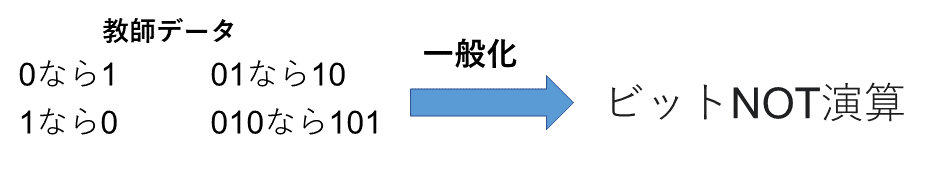
\includegraphics[width=90mm]{summary.jpg}
        %\epsfile{file=ab0ex-mtphu.eps,width=90mm}
    \end{center}
    \capwidth=90mm %
    \caption{NP4Gの概要}
    \label{fig:summary}
\end{figure*}

\subsection{NP4Gの基本構造}
%\subsection{NP4Gの構造}
\label{sec:struct}
NP4Gは\ref{fig:sequence}のように,複数の関数やオブジェクトといったノードがネットワーク状に接続された有効グラフ構造を持つ.
ノードは関数(図中の四角),プログラムの最初に実行されるスタートノード(図中の「S」と書かれた丸),プログラムの終了を知らせるエンドノード(図中の「E」と書かれた丸),入力のリンクがなく,予め格納されるデータを出力するオブジェクトノード(図中の丸)に大別される.スタートノードから順にノードが処理されていくことで,「順次」を実現できる.
入力として接続されるリンクの数は関数によって異なるが,出力のリンクの数は関数によらず何本でも接続できる.
\subsubsection{ノードの実行順序}
%\subsubsection{ネットワークの自動生成}
\label{sec:sequence}
ここで,NP4Gで生成されるネットワークの一例を示し,ノードの実行順序を説明する.
\ref{fig:sequence}に示すように,まずはじめに,入力データを持つスタートノードに接続されているノードが,上から順に実行される.それらのノードがすべて実行されたら,それらのノードに接続されているノードも同様に上から順に実行される.ネットワークをデータ系列として捉えた場合,この操作は,次に実行されるノードをリストとして並べ,前から順に実行する操作であるといえる.
\ref{fig:sequence}の\textcircled{\scriptsize 4}のように,まだ入力のノードからの出力がない場合,「not yet」となり,出力されない.これは,\textcircled{\scriptsize 9}のように,スタートノードから派生しないノードがあった場合,実行されないことを意味する.また,\textcircled{\scriptsize 8}のように,すでに実行されているノードは,「already done」となり,再び計算されることはない.このようにして,次に処理されるノードがなくなるまで,各ノードが実行される.最終的に,最後に実行されたノードの出力が,そのネットワーク全体の出力となり,エンドノードに接続される.すなわち,エンドノードは元からネットワークに接続されているのではなく,ノードの実行順序の関係から事後的に決められる.

\begin{figure*}[t]
    \begin{center}
        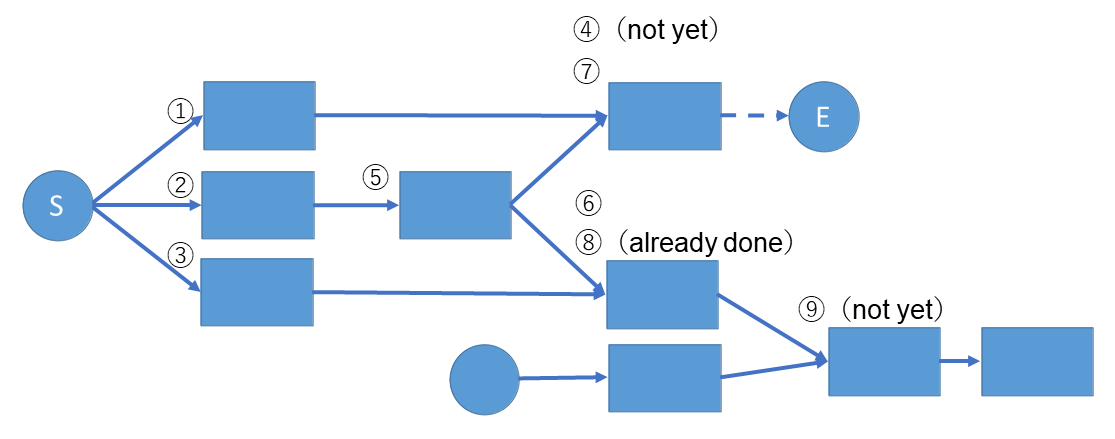
\includegraphics[width=130mm]{sequence.png}
    \end{center}
    \capwidth=90mm %
    \caption{NP4Gの実行順序}
    \label{fig:sequence}
\end{figure*}

\subsubsection{繰り返し処理}
%より表現力の高い計算モデルを構築するためには
構造化定理を満たすには,繰り返し処理を導入する必要がある.NP4Gでは,繰り返し処理をネットワーク上にフィードバックループを設けることで実現するのではなく,イテラブルなデータを関数に入力させることで実現する.入力としてイテラブルなデータが与えられた関数は,そのデータの要素ごとに同じ処理を実行する.
イテラブルなデータの生成あるいはイテラブルでないデータに戻す処理も関数が行い,イテラブルなデータが関数の入力として用いられる限り繰り返し処理がなされる.
こうすることで,無限ループに陥り終了することのないプログラムが作成されることなく繰り返し処理を実現することができる.また,ノードをランダムに組み合わせて,プログラムを自動生成する際にも,ノードの実行順序が簡潔になる分,エラーを起こしにくくなる.

\subsubsection{自動定義関数(ADFs)}
GPでは,プログラムの進化の際に高速化が望めるなどの理由から自動定義関数(ADFs: Automatically Defined Functions)が用いられる\cite{adfs}.ADFsにより,すでに出来上がったネットワークを再利用することで,より高度なプログラムを短時間のうちに作成することが可能になる.
%ADFsはGPの性能を向上させる目的で,プログラムに存在するモジュール性を利用する方法である.
NP4Gでは,ADFsを\ref{sec:PL}で説明する段階的学習と組み合わせ,段階ごとにADFsとしてネットワークを登録し,次の段階でそのネットワークを再利用できるようにする.

\subsubsection{段階的学習}
\label{sec:PL}
段階的学習(Phased Learning)は学習を各段階に分けて行うことで,複雑なプログラムであっても無理なく学習させる手法である.段階的学習は主に強化学習で用いられる手法であり,人工知能の取り得る自由度を下げることで,学習時間が膨大になるのを防ぐ効果がみられる\cite{hodohara2012reinforcement}.
NP4Gでは,まずは学習させる教師データの数を少なくし,簡単な処理を行うネットワークを生成させるところから始め,ADFsとして次にネットワークを構築するときのノードとして再利用させる.こうすることで,はじめから複雑なネットワークを得るときよりも短時間で学習をすることが期待できる.

\section{ビットNOT演算プログラムの獲得}
NP4Gを使って,ビットNOT演算プログラムを自動で構築する場合を考え,実際にNP4Gのプログラムを実行することで検証を行った.
%\subsection{設定}
%NP4Gを用いて,ビットNOT演算プログラムを獲得する実験を行った.
本研究ではプログラミング言語であるPython(Python 3.7.12)を使って,NP4Gのプログラムを作成した.実行環境として,GoogleのColaboratoryを使用した.
また,繰り返し処理を実現するためのイテラブルなデータとして,Pythonプログラム上でリスト型のオブジェクト(以下,リスト)を使用した.
NP4Gにおいて,教師データやスタートノード,オブジェクトノードに格納されるデータはすべて文字列である.

\subsection{予め与えられる関数}
ネットワークを構築するための関数として,予め与えられるノードは,\ref{fig:func}に示すように,split関数,sum関数,equal関数,制御ゲート関数の4つである.以下,それぞれの関数の内容を説明する.
\subsubsection{split関数}
スペースを区切りとして,文字列を分けリスト表記にする.図で示すときは「split」を四角で囲い表記する.

%\begin{figure}[t]
%    \begin{center}
%        %\includegraphics[width=90mm]{ab0ex-mtphu.eps}
%        \includegraphics[width=50mm]{div.png}
%        %\epsfile{file=ab0ex-mtphu.eps,width=90mm}
%    \end{center}
%    \capwidth=50mm %
%    \caption{図の説明文... }
%\end{figure}

\subsubsection{sum関数}
リスト型の入力やそれ以外の文字列など,複数の入力に対し平滑化を行い,文字列との間をスペースで挟んで結合することで1つの文字列にする.入力の文字列が"[NULL]"である場合,"[NULL]"は結合しない.出力の文字列が""である場合,"[NULL]"を出力する.図で示すときは「+」を四角で囲い表記する.

\subsubsection{equal関数}
2本の入力の値が一致するとき"[TRUE]"を出力する.それ以外は"[FALSE]"を出力する.GP/GNPにおける判定ノードの役割を果たす.図で示すときは「==」を四角で囲い表記する.

\subsubsection{制御ゲート関数}
2本の入力のうち,どちらかが"[TRUE]"である場合は,もう片方の入力の値を通し,それ以外は"[NULL]"を出力する.GP/GNPにおける処理ノードの役割を果たす.図で示すときは白丸で表記する.

\begin{figure*}[t]
    \begin{center}
        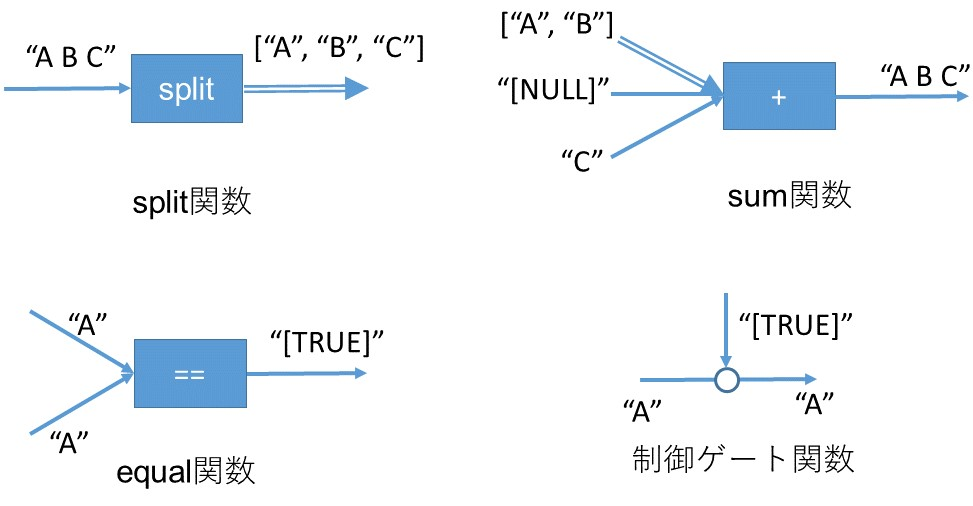
\includegraphics[width=110mm]{func.jpg}
    \end{center}
    \capwidth=90mm %
    \caption{予め与えられる関数}
    \label{fig:func}
\end{figure*}

\subsection{ビットNOT演算プログラムの例}
これらの関数を用いることで実現されるビットNOT演算プログラムの例を\ref{fig:bitwise_not}に示す.このように,例えば,はじめに論理NOTプログラムをネットワークとして構築する.次に,このネットワークをADFsとして次のネットワークの構築に再利用できる形にする.最後に,イテラブルなデータ(リスト)の繰り返し処理によって,個々の要素に対してADFsである論理NOTを適応することで,ビットNOT演算プログラムを得る.このように段階を踏んでネットワークを構築する段階的学習を行うことで,目的のプログラムを実現する.

\begin{figure*}[t]
    \begin{center}
        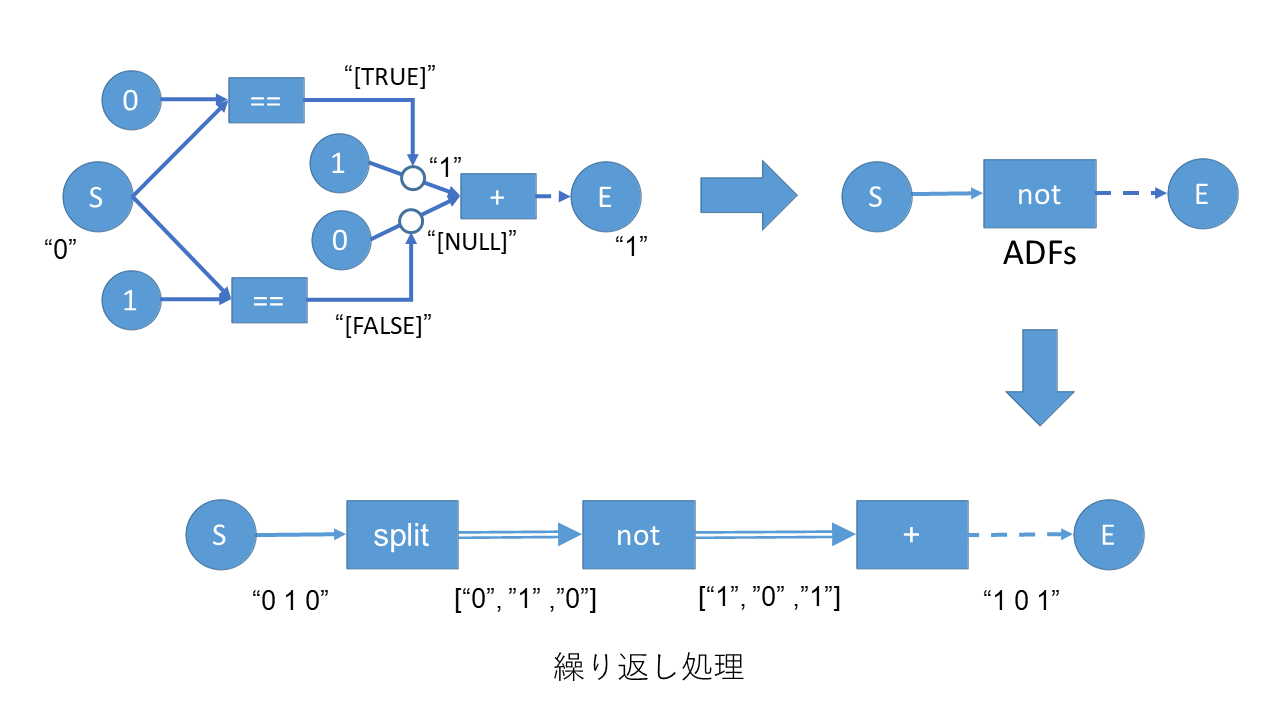
\includegraphics[width=150mm]{bitwise_not.png}
    \end{center}
    \capwidth=130mm %
    \caption{ビットNOT演算プログラムの実現例.このように段階を踏んでネットワークを構築することで,目的のプログラムを実現する(段階的学習).ADFsにより,最初に作った論理NOTプログラムのネットワークを次のネットワーク構築に再利用する.繰り返し処理はイテラブルなデータ(リスト)によって行われる.}
    \label{fig:bitwise_not}
\end{figure*}

\subsection{検証方法}
本研究で用いる教師データは,\ref{tbl:TeacherData}に示す4つであり,段階的学習の方法によって,各段階で使われる教師データが変わる.なお,教師データのそれぞれの入出力は(入力,出力)のように括弧書きで表記する.

\begin{table}[htbp]
\centering
\caption{本研究で用いる教師データのすべて}
\label{tbl:TeacherData}
\begin{tabular}{l}
    \hline
     ( 入力 , 出力 ) \\
    \hline \hline
    ( "0" , "1" ) \\
    ( "1" , "0" ) \\
    ( "0 0" , "1 1" ) \\
    ( “0 1 0” , ”1 0 1” ) \\
    \hline
\end{tabular}
\end{table}

本研究では,NP4Gによるプログラムの自動生成として,各段階のこれらの教師データに合致するようなネットワークを,ノードをランダムに組み合わせることで探索する.そのランダムアルゴリズムは,まず決められたノード数だけランダムにノードを選び,次に関数の入力の数だけランダムに他のノードと繋ぐものである.
本研究の検証では,ビットNOT演算プログラムを自動で構築するプログラムを10回実行し,その生成結果と実行時間の平均値を求めた.生成結果の記述は,探索して得られたネットワークが,期待するプログラムが得られるネットワークであれば「成功」,そうでない場合は「失敗」,1回のプログラムの実行における制限時間内に生成されなかった場合は「超過」とする.
1回のプログラムの実行における制限時間は3時間(10800秒)とした.
1桁から5桁までのすべての2進数の文字列(”0”から”1 1 1 1 1”)を使って,生成されたプログラムを検証した.
なお,スタートノードとエンドノードの数はノード数に含まれない.

\subsubsection{段階的学習の方法}
\label{sec:PLhow}
本研究では,段階的学習で用いる段階を段階1から段階5まで用意し,それぞれの段階の組み合わせを変えることで,段階的学習の影響を調べた.段階的学習で用いる5つの段階の教師データは以下の通りである.

%1. “0”の入力に対して”1”の出力

%2. ”1”の入力に対して“0”の出力

%3. “0”の入力に対して”1”の出力,”1”の入力に対して“0”の出力

%4. “0”の入力に対して”1”の出力,”1”の入力に対して“0”の出力,“0 0”の入力に対して”1 1”の出力

%5. “0”の入力に対して”1”の出力,”1”の入力に対して“0”の出力,“0 0”の入力に対して”1 1”の出力,“0 1 0”の入力に対して”1 0 1”の出力

段階1. (“0”,”1”)

段階2. (”1”,“0”)

段階3. (“0”,”1”), (”1”,“0”)

段階4. (“0”,”1”), (”1”,“0”), (”0 0”,“1 1”)

段階5. (“0”,”1”), (”1”,“0”), (”0 0”,“1 1”), (”0 1 0”,“1 0 1”)

これらの各段階を,段階2,3,4の3段階,段階1,2,3,4の4段階,段階1,2,3,4,5の5段階と段階の数を変えて比較することで,段階的学習の影響を調べる.
本研究では,NP4Gによるプログラムの自動生成として,各段階のこれらの教師データに合致するようなネットワークを,予め与えられるノードとADFsをランダムに組み合わせることで探索する.
各段階で得られたネットワークは,Pythonのラムダ式を使ってADFsとしてリストに追加することで,次の段階で再利用可能にする.
なお,各段階で学習に用いられる教師データの文字列は,ネットワークを構築するためのオブジェクトノードとして,予め与えられる.

\section{結果と考察}
3段階から5段階まで段階的学習の段階の数を変化させたときの生成結果と実行時間の結果を\ref{tbl:result1},\ref{tbl:result2},\ref{tbl:result3}に示す.また,各段階における平均時間の結果を\ref{tbl:result4}に示す.

3段階から5段階までのすべての生成結果を見ると,失敗したネットワーク(教師データの条件はすべて満たすが検証結果を満たさない)は段階的学習が4段階,ノード数が10個のときの1例のみだった.時間内に終わりやすいのは,段階的学習が3段階,ノード数が10個のときだった.
ノード数5のときの生成結果を見ると,5段階のときの成功の1例のみを除いて,すべて時間超過となった.\ref{fig:out_net_p5n5}に5段階ノード数5での自動生成によって期待するプログラムが得られたときのネットワークを示す.このネットワークのように,ノード数が少ない場合でも,期待するネットワークが得られることがわかった.
このネットワークの場合,段階4の時点でビットNOT演算プログラムが得られていることを確認している.このように,段階的学習の途中でも期待するネットワークが得られることがわかった.
\ref{fig:out_net_p4n10}に4段階ノード数10での自動生成によって,学習に用いた教師データと入出力は一致したが,期待と異なるプログラムが得られたときのネットワークを示す.このネットワークの場合,”0 1 0”の入力に対して“0 1 1”となり,“1 0 1”でない出力となった.このように,教師データと入出力が一致するネットワークが生成されたとしても,期待するネットワークが得られない場合もあることがわかった.この場合でも,段階を増やし,(”0 1 0”,“1 0 1”)の教師データも含めた教師データによって学習することで,期待するネットワークが得られると考えられる.また,ネットワークを構築する際はランダムにノードを選択するため,\ref{fig:out_net_p4n10}の段階2や段階4からも,必ずしも前の段階で生成されたADFsであるadf1やadf3を使うとは限らないことがわかる.
\ref{tbl:result4}からわかるように,段階3の学習時間が2585.24(s)と最も高くなっている.この原因は,段階3が「(“0”,”1”), (”1”,“0”)」の学習であり,1つのネットワークで初めて,2つの条件を満たすネットワークを探索する必要があることから,学習コストが高くなったためと考えられる.

%\begin{table}[htbp]
%\centering
%\begin{center}
%\end{tabular}
%\end{center}
%\end{table}

\begin{table}[t]
\caption{3段階の段階的学習の生成結果と実行時間(s)}
\label{tbl:result1}
\begin{tabular}{c|cccc}
    ノード数&	5&	10&	15&	20\\
    \hline \hline
    成功&	0&	8&	6&	2\\
    失敗&	0&	0&	0&	0\\
    超過&	10&	2&	4&	8\\
    \hline
    平均時間&	- &	3067.23&	5564.88&	3699.22\\
    最大時間&	- &	10480.28&	8966.41&	9542.54\\
    最小時間&	- &	258.23&	1.19&	3.24\\
    \hline
\end{tabular}
\end{table}

\begin{table}[t]
\caption{4段階の段階的学習の生成結果と実行時間(s)}
\label{tbl:result2}
\begin{tabular}{c|cccc}
    ノード数&	5&	10&	15&	20\\
    \hline \hline
    成功&	0&	7&	6&	7\\
    失敗&	0&	1&	0&	0\\
    超過&	10&	2&	4&	3\\
    \hline
    平均時間&	-&	3023.63&	334.40&	1104.84\\
    最大時間&	- &	8293.86&	1102.60&	2834.49\\
    最小時間&	- &	133.70&	6.46&	9.77\\
    \hline
\end{tabular}
\end{table}

\begin{table}[t]
\caption{5段階の段階的学習の生成結果と実行時間(s)}
\label{tbl:result3}
\begin{tabular}{c|cccc}
    ノード数&	5&	10&	15&	20\\
    \hline \hline
    成功&	1&	6&	7&	5\\
    失敗&	0&	0&	0&	0\\
    超過&	9&	4&	3&	5\\
    \hline
    平均時間&	32.18&	4089.67&	1505.77&	1265.54\\
    最大時間&	32.18&	9103.33&	7866.33&	2585.50\\
    最小時間&	32.18&	0.75&	2.29&	26.04\\
    \hline
\end{tabular}
\end{table}

\begin{table}[t]
\caption{各段階における平均時間(s)}
\label{tbl:result4}
\begin{tabular}{c|ccccc}
    段階&	1&	2&	3&	4&	5\\
    \hline
    平均時間&	1.17&	2.24&	2585.24&	188.31&	12.49\\
\end{tabular}
\end{table}


%\begin{figure*}[t]
%    \begin{center}
%        %\includegraphics[width=90mm]{ab0ex-mtphu.eps}
%        \includegraphics[width=120mm]{network.jpg}
%        %\epsfile{file=ab0ex-mtphu.eps,width=90mm}
%    \end{center}
%    \capwidth=90mm %
%    \caption{図の説明文... }
%    \label{fig:net}
%\end{figure*}

\begin{figure*}[t]
    \begin{center}
        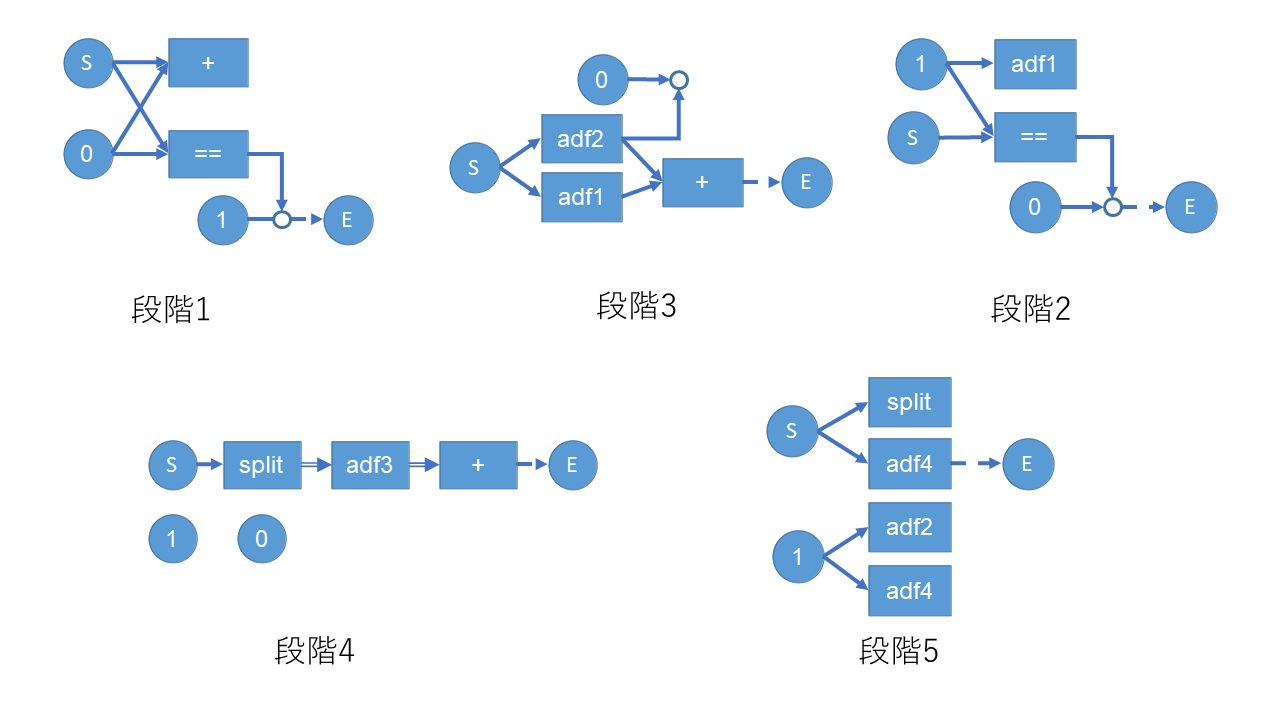
\includegraphics[width=150mm]{out_net_p5n5.png}
    \end{center}
    \capwidth=90mm %
    \caption{5段階ノード数5での自動生成によって期待するプログラムが得られたときのネットワーク}
    \label{fig:out_net_p5n5}
\end{figure*}

\begin{figure*}[t]
    \begin{center}
        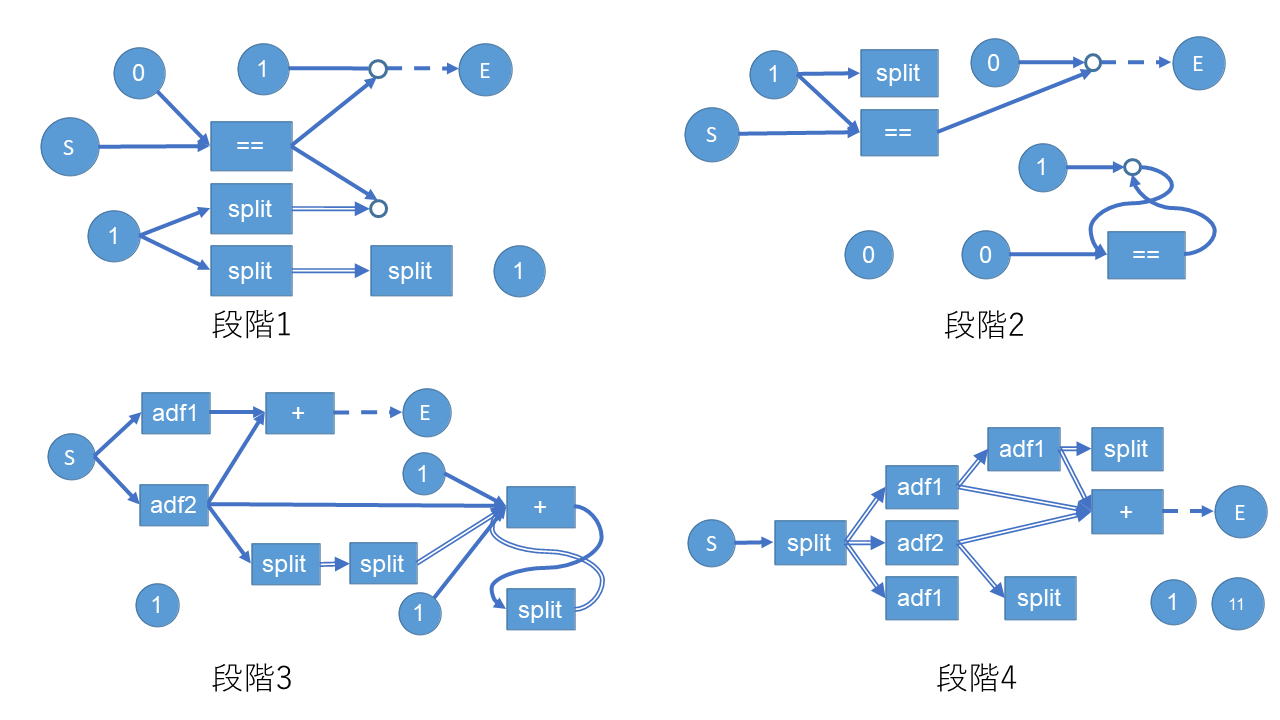
\includegraphics[width=150mm]{out_net_p4n10.png}
    \end{center}
    \capwidth=90mm %
    \caption{4段階ノード数10での自動生成によって,学習に用いた教師データと入出力は一致したが,期待と異なるプログラムが得られたときのネットワーク}
    \label{fig:out_net_p4n10}
\end{figure*}

\section{おわりに}
\subsection{まとめと本研究の意義}
本研究では,一般化のためのネットワークプログラミング(NP4G)を提案した.NP4Gを使うことで,数個の教師データからビットNOT演算プログラムを獲得できることを確認した.
NP4Gは,数個の事例から一般的な性質を見出していく手法であるため,帰納推論である.
また,プログラミングにおける「順次」,「選択」,「繰り返し」の,構造化定理の条件を満たす構造になっており,任意プログラムを帰納推論によって自動的に獲得することが期待できる手法である.
NP4Gによって示された,遺伝的手法に限らないネットワークプログラミング(NP)は,新しい自動プログラミングの手法として,今後新しい分野として幅広く応用されると期待できる.
本研究の意義は,ネットワークプログラミング(NP)によって,あらゆる知識に対し自ら学習をし,その内容を活かして別の問題に対して論理的に推論し答えを導くような,汎用的で柔軟な人工知能の実現が期待できることを示した点にある.
\subsection{今後の課題}
\subsubsection{チューリング完全性}
NP4Gは構造化定理の条件を満たすことを説明したが,NP4Gが任意のプログラムを得られる手法であることを証明するためには,NP4Gがチューリング完全であることを示す必要がある.チューリング完全とは,ある計算モデルが万能チューリングマシンと同等の計算能力を持つ,すなわち,任意のプログラムを再現することができることを示すものである.
チューリング完全であることが示されれば,帰納推論により任意のプログラムを獲得できる手法が実現できたことを意味する.
%広く自動プログラミングとして応用可能であることが理論的に示すことができる.
また,ビットNOT演算子だけでなく,他のプログラムもNP4Gを使って自動で構築できるか実際に試してみる必要がある.
\subsubsection{探索手法の模索}
本研究では,ネットワークの探索方法として,ランダムな生成による偶発的な探索手法を用いた.
%この手法はプリミティブな手法であり,より効率の良い探索手法を模索する余地が残る.
この手法はプリミティブであるがゆえに,用いるノードの種類や数が増えたり,目的のプログラムが複雑であるほど,探索に時間がかかる.
今後,強化学習を用いるなど,他の学習手法と組み合わせることで,ネットワークの構成要素として相応しいノードの種類や数,組み合わせ方を自動で調整し,ネットワーク構築の効率化を図る必要がある.
\subsubsection{ネットワークの評価}
遺伝的手法や強化学習など,他の学習手法では,生成されたネットワークやモデルを,評価関数を用いて数値評価する機構が備わっている.本研究では,目的のネットワークが生成されたか否かの評価となっており,評価関数による数値評価ができていない.今後,NP4Gでのネットワークの評価方法を確立できれば,ネットワークの評価によって,構築の仕方を変えたりすることもできる.また,評価関数を用いる他の学習手法とも組み合わせしやすくなる.
\subsubsection{生成されたネットワークの簡素化}
\ref{sec:sequence}でも説明したように,NP4Gではネットワークにノードがあったとしても,スタートノードから派生するノードでない場合,そのノードは実行されることがない.このようなノードが出てきた場合,ネットワークを生成したあとで取り除くようなアルゴリズムが提案されれば,生成されたネットワークの簡素化を図ることができる.
\begin{acknowledgment}
本研究は,JST次世代研究者挑戦的研究プログラム JPMJSP2130 の支援を受けたものである.
\end{acknowledgment}

\bibliography{btx_np4g}
\bibliographystyle{jsai}

%\appendix
%\section{付録のタイトル1}
%付録の本文1
%\section{付録のタイトル2}
%付録の本文2

% 著者の姓と名の間は半角スペースで区切る
% 略歴は200字以内
\begin{biography}
\profile{s}{原 匠一郎}{2018年3月名城大学理工学部電気電子工学科卒業.2020年3月名古屋市立大学大学院システム自然科学研究科博士前期課程 修了.現在,名古屋市立大学大学院理学研究科博士後期課程在籍中.情報処理学会会員.}
\profile{n}{渡邊 裕司}{著者2の略歴}
%\profile*{m}{著者姓 名}{前掲\kern-.5zw (Vol.X,No.Y,p.Z)\kern-.5zw 参照.}
\end{biography}

\end{document}
